%%%%%%%%%%%%%%%%%%%%%%%%%%%%%%%%%%%%%%%%%%%%%%%%%%%%%%%%%%%%%%%%%%%%%%%%%%%%%%%%
\subsection{2D Lucas-Kanade Alignment of 2.5D Images}\label{subsec:singl_img_lk_2d}
%%%%%%%%%%%%%%%%%%%%%%%%%%%%%%%%%%%%%%%%%%%%%%%%%%%%%%%%%%%%%%%%%%%%%%%%%%%%%%%%
In this section we propose to use normals as a robust descriptor for the
alignment of 2.5D depth data. As previously discussed, 2.5D data provides a depth
or height value per-pixel in the image domain and thus is discretised into
a 2D image. Therefore, construction of a Lucas-Kanade algorithm for the alignment
of depth data follows directly form the Lucas-Kanade algorithm descriptions
outlined in the previous section. The only difference is that, instead of
computing the SSD error on the colour or grayscale pixel data we instead compute
the SSD error on the depth values.

In order to augment the classical Affine Lucas-Kanade algorithm to use normals
we follow the methodology proposed by \citet{antonakos2015feature}. That is,
we treat the normals as a feature that is extracted from the depth values
and linearise the feature as though it were a multi-channel input. In this case,
the vector valued SSD error described in the previous section simply
becomes the concatenation of all of the channels of the multi-channel
``feature image''. Specifically, in the case of normals, we would assume
that the input image $I$ becomes $f(I)$ where
$f(I) = {[n^x_1, n^y_1, n^z_1, \ldots, n^x_D, n^y_D, n^z_D]}^T$ is defined as
the feature extraction function that computes the surface normals from the
image. Given that no statistical model of appearance is employed in Affine
Lucas-Kanade, using the normals directly as feature is equivalent to
the inner product kernel described in \cref{subsubsec:sing_img_ip_kernel}.
More explicitly, we define two new feature description methods which are
restated from our kernels described in \cref{subsubsec:singl_img_ca_kpca}.
We provide the following definitions which are defined to operate on a single
depth pixel for simplicity:
%%%%%%%%%%%%%%%%%%%%%%%%%%%%
\begin{equation}
    \begin{aligned}\label{eq:normal_feature_functions}
        f_{\ipname}(i)    &= {[n_x, n_y, n_z]}^T \\
        f_{\sphername}(i) &= {[\cos \phi, \sin \phi, \cos \theta, \sin \theta]}^T
    \end{aligned}
\end{equation}
%%%%%%%%%%%%%%%%%%%%%%%%%%%%
where
%%%%%%%%%%%%%%%%%%%%%%%%%%%%
\begin{equation}
    \begin{aligned}\label{eq:normalised-spherical}
        \cos \phi   &=& \tilde{n_x} \;\;\;\; \sin \phi   &=& \tilde{n_y} \\
        \cos \theta &=& \tilde{n_z} \;\;\;\; \sin \theta &=& \sqrt{1 - {\tilde{n_z}}^2}
    \end{aligned}
\end{equation}
%%%%%%%%%%%%%%%%%%%%%%%%%%%%
and $\tilde{n_x} = \frac{n_x}{\sqrt{n_x^2 + n_y^2}}$,
$\tilde{n_y} = \frac{n_y}{\sqrt{n_x^2 + n_y^2}}$,
$\tilde{n_z} = \frac{n_z}{\sqrt{n_x^2 + n_y^2 + n_z^2}}$.
This normalisation of each component is done to suppress any magnitude
contribution from orientation.

\textbf{Applicability of the AEP and PGA kernel to parametric image alignment.}
Although it is simple to define our proposed kernels as descriptors suitable
for parametric image alignment, this is not the case for the
AEP~\cite{smith2006recovering} and PGA~\cite{smith2008facial} projection
operations. Firstly, we note that both the AEP and PGA operators are identical
in their mapping function with the primary difference being in the computation
of the per-pixel mean estimate required for computing the tangent plane. This
is in contrast to our proposed kernels which are independent per-pixel. This
reliance on a mean estimate for computing the differences is precisely what
makes these operations unsuitable for alignment. In the case of template based
Lucas-Kanade it is unclear where the estimate of the mean should computed as
only a single image is provided as a template and therefore a mean cannot
be computed. Furthermore, even if a mean is constructed from a training set
consisting of a single individual, it is highly likely that the deviation
from this mean face for a given input image will be very close to this mean. This
means that the distance from the neutral template image and the likely neutral
mean will be extremely small. In fact, in the worst case where the neutral does
not deviate from the mean neutral face at all the template image in ``feature''
space would be completely zero. This is because there is zero distance in
the tangent plane between the mean estimate and the template. Furthermore,
since the tangent projection already measures a distance, this means that
the similarity between the template and the current estimate is not well
described by the feature. For these reasons, we do not consider the AEP or PGA
kernels in the following parametric alignment investigation.

As discussed, we also propose to use the AAM extension of the classical
Affine Lucas-Kanade algorithm as proposed by \citet{matthews2004active}.
Therefore, the remainder of the section describes how to construct an AAM
using a multi-channel image.
%%%%%%%%%%%%%%%%%%%%%%%%%%%%%%%
\subsubsection{Lucas-Kanade AAMs}\label{subsubsec:2d-lk-aams}
%%%%%%%%%%%%%%%%%%%%%%%%%%%%%%%
An AAM is defined by a shape, appearance and a motion model. The shape model is
typically learnt by annotating $N$ fiducial points, $\bb{s} = [x_1, y_1,
\ldots, x_N, y_N]^T$ on each image in a set of training images. PCA is then
applied to these points and the shape, $\bb{s}$, can be expressed as a
base shape $\bb{s}_0$ plus a linear combination of $P$ shape vectors,
$\bb{s}_i$:
%%%%%%%%%%%%%%%%%%%%%%%%%%%%
\begin{equation}\label{eq:aam-shape-model}
    \bb{s} = \bb{s}_0 + \sum^P_{i=1} p_i \bb{s}_i
\end{equation}
%%%%%%%%%%%%%%%%%%%%%%%%%%%%
where $p_i$ are the shape coefficients.
An example of an AAM shape model is given in \cref{fig:singl_img_aam_shape_model}.
The appearance model is learnt by first
warping each training image to the reference frame defined by $\bb{s}_0$
to yield a set of shape-free textures. Each image is warped using an appropriate
non-rigid warping function such as piecewise affine \cite{cootes2001active} or thin
plate splines \cite{papandreou2008adaptive}. PCA is applied to the shape-free textures to
yield a set of $M$ appearance vectors. The appearance vectors are defined for
each pixel inside $\bb{s}_0$ when $\p = \zero$. Therefore, the
appearance, $A_\lambda(\zero)$, can be expressed as a base appearance,
$A_0(\zero)$, plus a linear combination of $M$ appearance vectors:
%%%%%%%%%%%%%%%%%%%%%%%%%%%%
\begin{equation}\label{eq:aam-appearance-model}
    A_{\blambda}(\zero) = A_0(\zero) + \bb{A} \blambda
\end{equation}
%%%%%%%%%%%%%%%%%%%%%%%%%%%%
where $\bb{A} = [A_1(\zero), \ldots, A_M(\zero)]$, the matrix of
concatenated appearance vectors, $\blambda = [\lambda_0, \ldots, \lambda_M]^T$,
the vector of appearance parameters, and thus $\bb{A} \blambda =
\sum^M_{i=1} \lambda_i A_i(\zero)$. Given a test image, $I$, fitting an AAM
entails estimating the parameters $\p = [p_0, \ldots, p_P]^T$ and $\blambda$.
Formally, the AAM objective function is
%%%%%%%%%%%%%%%%%%%%%%%%%%%%
\begin{equation}\label{eq:aam-objective}
    \argmin_{\p,\blambda} \norm{I(\p) - A_{\blambda}(\zero)}^2
\end{equation}
%%%%%%%%%%%%%%%%%%%%%%%%%%%%
A number of approaches have been proposed to minimise this objective function
\cite{gross2005generic,matthews2004active,papandreou2008adaptive}, the most popular of
which is the project-out inverse compositional algorithm (PIC)
\cite{cootes2001active,amberg2009compositional} due to its efficiency. Although efficient, PIC
is unable to perform well under unseen variation and therefore we have chosen to
use the alternating simultaneous approach described in \cite{matthews2004active}.
%%%%%%%%%%%%%%%%%%%%%%%%%%%%%%%%%%%%%%%%
\setlength{\tabcolsep}{2pt}
\begin{figure}
    \centering
    \resizebox{\textwidth}{!}{%
    \begin{tabular}{cccccc}
    Mean & PC 1 & PC 2 & PC 3 \\
    \multirow{3}{*}{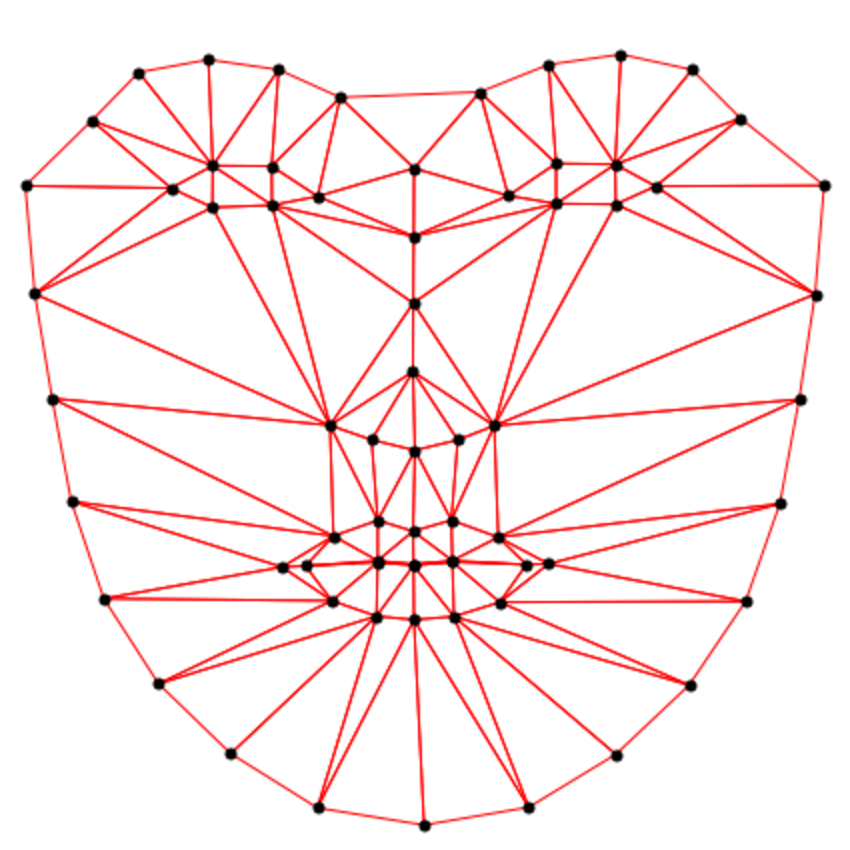
\includegraphics[valign=m,scale=0.16]{statistical_normals/images/lk2d/aam_shape_mean}} & 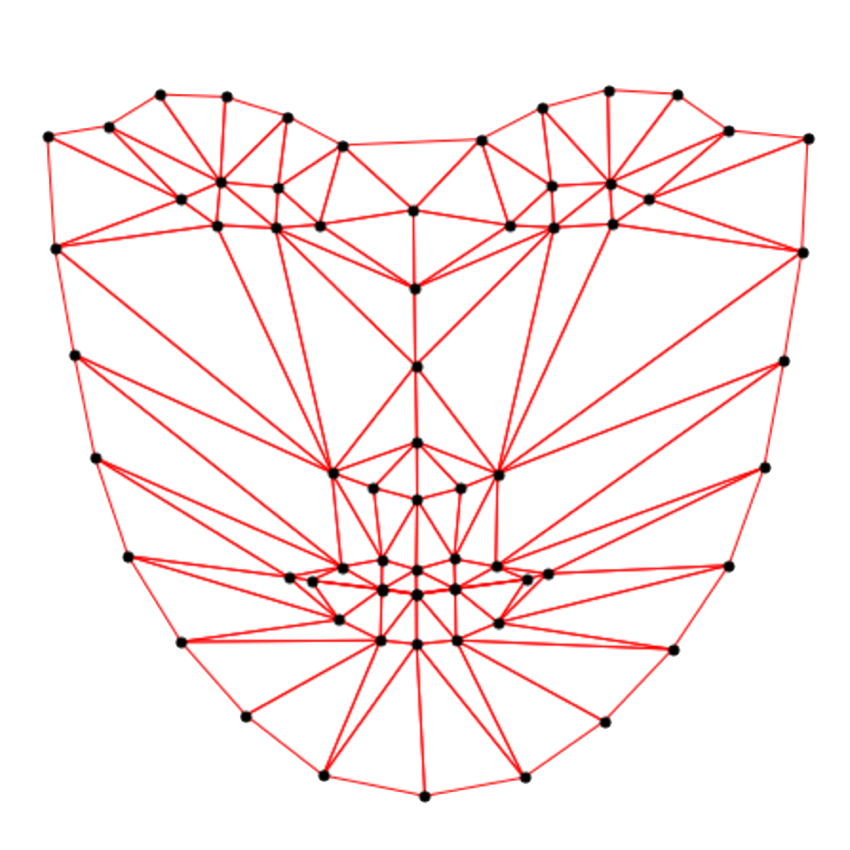
\includegraphics[valign=m,scale=0.16]{statistical_normals/images/lk2d/aam_shape_1_p3} & 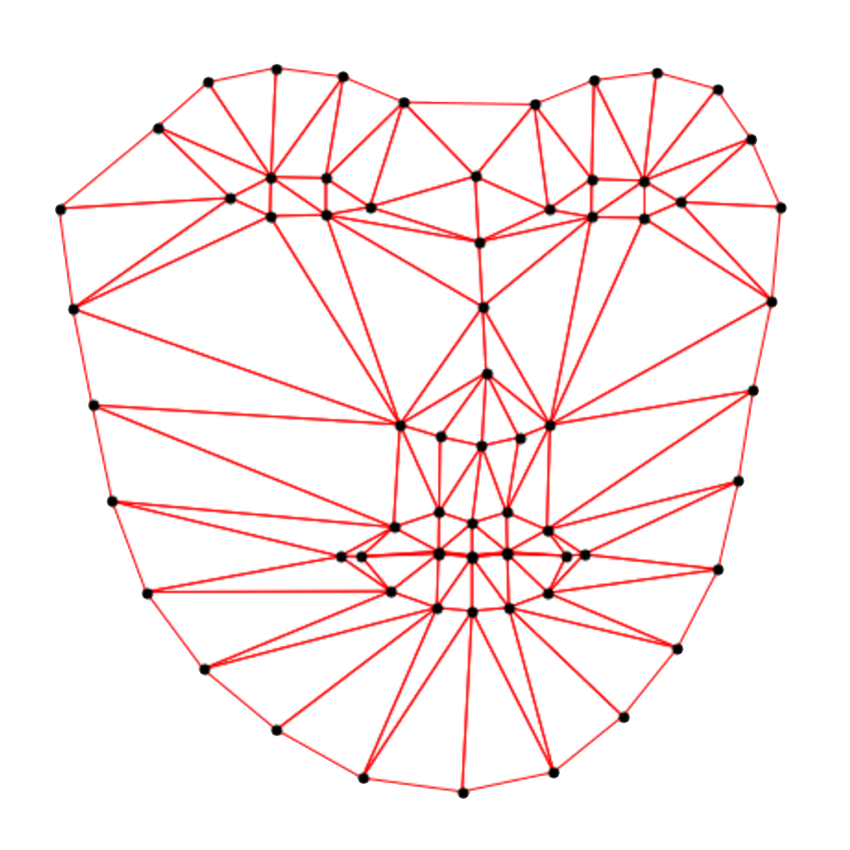
\includegraphics[valign=m,scale=0.16]{statistical_normals/images/lk2d/aam_shape_2_p3} & 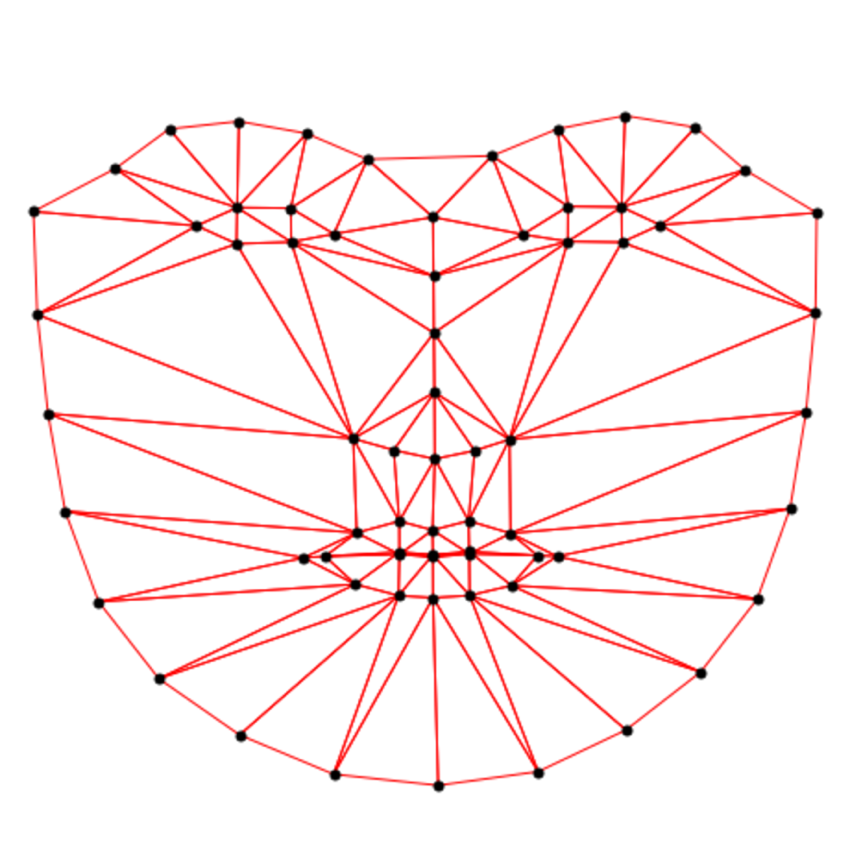
\includegraphics[valign=m,scale=0.16]{statistical_normals/images/lk2d/aam_shape_3_p3} \\
     & 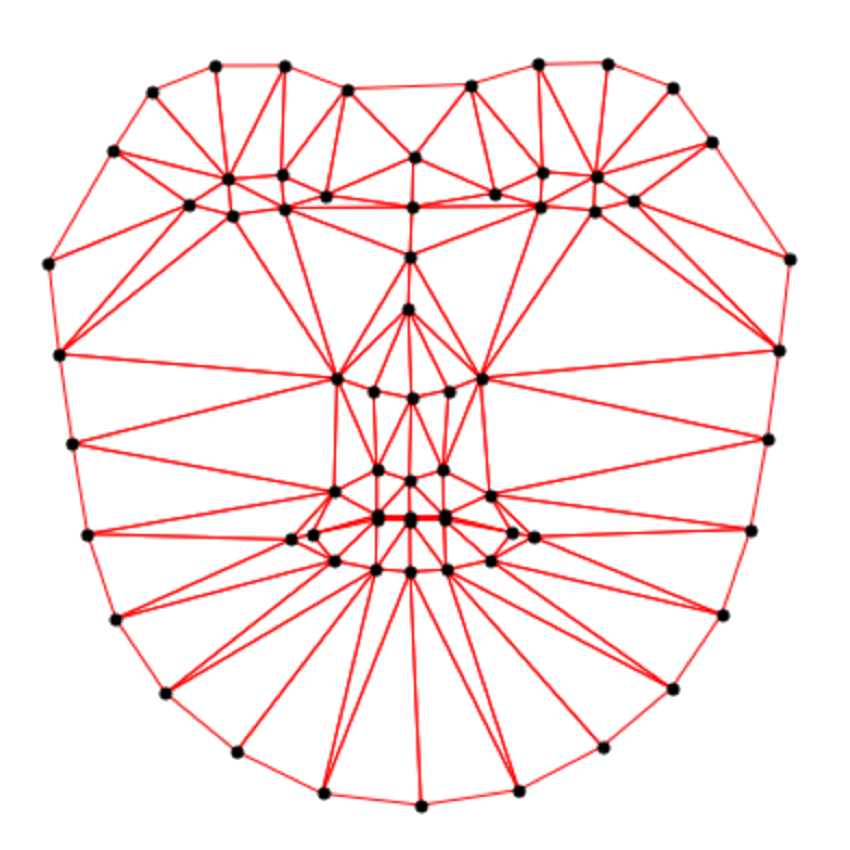
\includegraphics[valign=m,scale=0.16]{statistical_normals/images/lk2d/aam_shape_1_m3} & 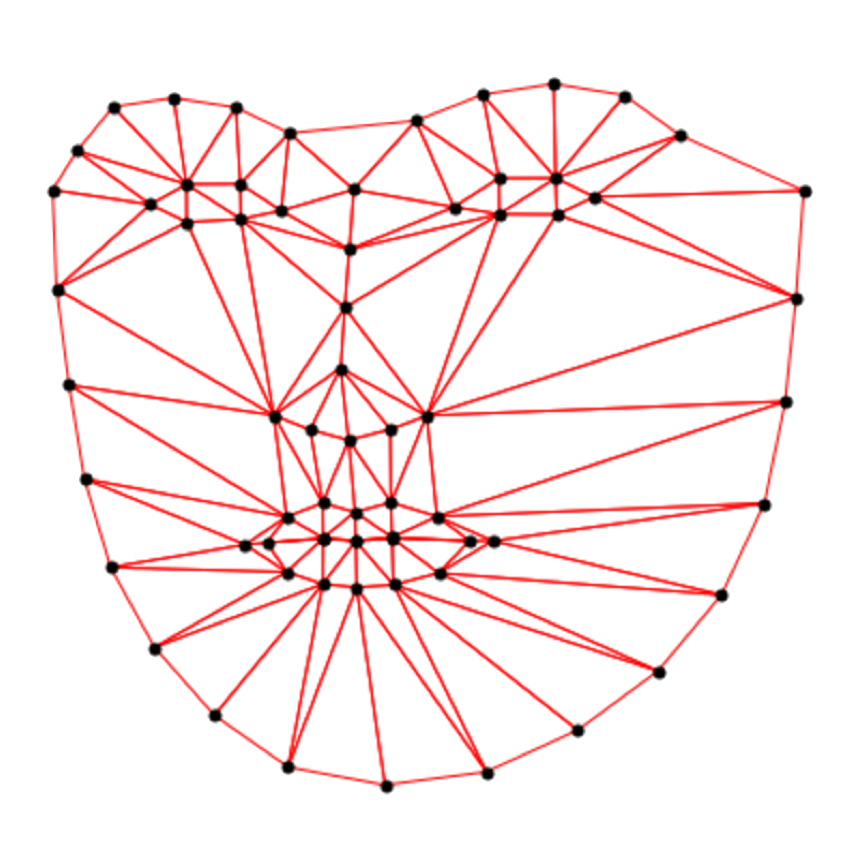
\includegraphics[valign=m,scale=0.16]{statistical_normals/images/lk2d/aam_shape_2_m3} & 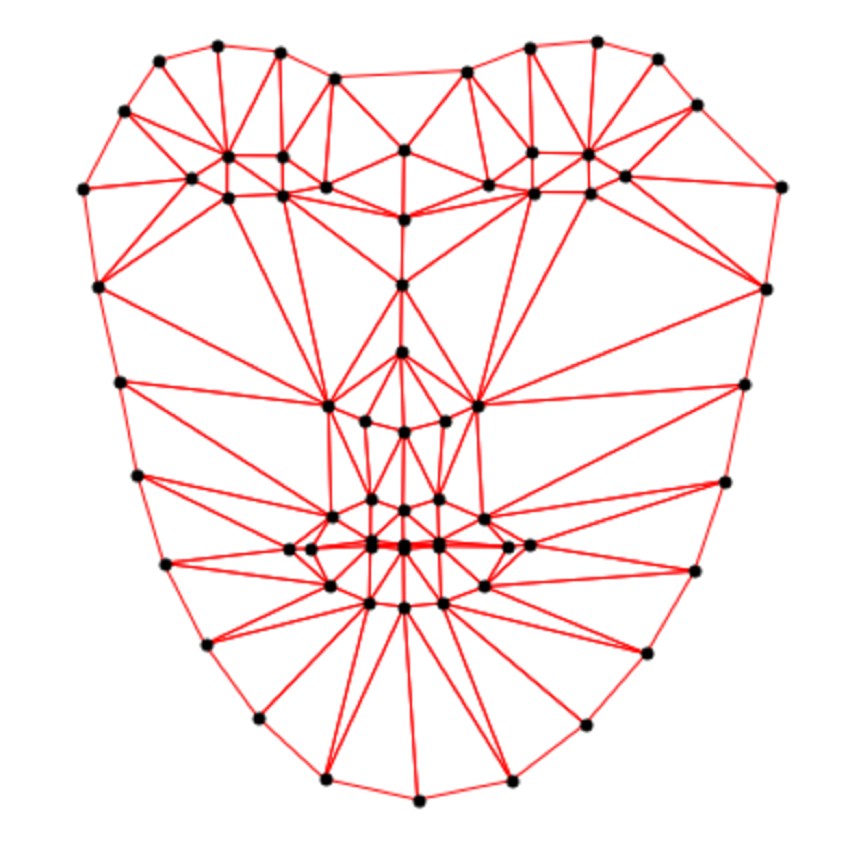
\includegraphics[valign=m,scale=0.16]{statistical_normals/images/lk2d/aam_shape_3_m3}
    \end{tabular}%
    }
    \caption{The PCA basis of facial deformation learnt from the
             2D annotations from the 300W~\cite{sagonas2013300} competition
             of the LFPW~\cite{belhumeur2013localizing} training images subset.
             The top and bottom rows show the principal components for
             $\pm 3 \sigma$ respectively.}
\label{fig:singl_img_aam_shape_model}
\end{figure}
\setlength{\tabcolsep}{6pt}
%%%%%%%%%%%%%%%%%%%%%%%%%%%%%%%%%%%%%%%%
%%%%%%%%%%%%%%%%%%%%%%%%%%%%%%%
\subsubsection{Simultaneous IC Algorithm}\label{subsec:aam-simultaneous}
%%%%%%%%%%%%%%%%%%%%%%%%%%%%%%%
The simultaneous algorithm \cite{gross2005generic} finds both the $\Delta \p$ and
$\Delta \blambda$ updates simultaneously. This involves iteratively solving for
$\Delta \p$ and $\Delta \blambda$ by linearising \cref{eq:aam-objective} such
that
%%%%%%%%%%%%%%%%%%%%%%%%%%%%
\begin{equation}\label{eq:aam-simultaneous-linearise}
    \argmin_{\Delta \p, \Delta \blambda} \norm{I(\p) - A_{\blambda}(\zero) - \frac{\partial A_{\blambda}(\zero)}{\partial \p} \Delta \p - \bb{A} \blambda}^2
\end{equation}
%%%%%%%%%%%%%%%%%%%%%%%%%%%%
Let $\Delta \bb{q} = [{\Delta \p}^T, {\Delta \blambda}^T]^T$ be the
concatenated vector of parameters. By performing a compositional update to the
warp parameters and an additive update to the appearance parameters, $\Delta
\bb{q}$ can be found simultaneously via
%%%%%%%%%%%%%%%%%%%%%%%%%%%%
\begin{equation}\label{eq:aam-simultaneous-deltaq-update}
    \Delta \bb{q} = \bb{H}_{\bb{q}}^{-1} \bb{J}_{\bb{q}}^{T} \left[ I(\p) - A_{\blambda}(\zero) \right]
\end{equation}
%%%%%%%%%%%%%%%%%%%%%%%%%%%%
where $\bb{H}_{\bb{q}} = \bb{J}_{\bb{q}}^{T}
\bb{J}_{\bb{q}}$ and $\bb{J}_{\bb{q}} = \left[
{\frac{\partial A_{\blambda}(\zero)}{\partial \p}}^T, \bb{A} \right]$.
Due to the additive update of the appearance parameters, $\blambda \leftarrow
\blambda + \Delta \blambda$, and thus the dependence of
$\bb{J}_{\bb{q}}$ on $\blambda$, the Jacobian and Hessian
matrices must be recomputed at each step. Although this is much less efficient
than the PIC algorithm, it has been shown to given excellent fitting performance
in practise.
%%%%%%%%%%%%%%%%%%%%%%%%%%%%%%%
\subsubsection{Alternating IC Algorithm}\label{subsec:aam-alternating}
%%%%%%%%%%%%%%%%%%%%%%%%%%%%%%%
The variation of the simultaneous inverse compositional algorithm proposed in
\cite{matthews2004active} solves for the shape and appearance updates in an
alternating manner, as
%%%%%%%%%%%%%%%%%%%%%%%%%%%%
\begin{equation}
    \begin{aligned}\label{eq:aam-alternating}
        \Delta \tilde{\p} &=       \argmin_{\Delta \p}       \norm{I(\p) - A_{\blambda}(\zero) - \frac{\partial A_{\blambda}(\zero)}{\partial \p} \Delta \p}^2_{\bb{I} - \bb{A} \bb{A}^T} \\
        \Delta \tilde{\blambda} &= \argmin_{\Delta \blambda} \norm{I(\p) - A_{\blambda}(\zero) - \frac{\partial A_{\blambda}(\zero)}{\partial \p} \Delta \tilde{\p} - \bb{A} \Delta \blambda}^2
    \end{aligned}
\end{equation}
%%%%%%%%%%%%%%%%%%%%%%%%%%%%
where $\bb{I} - \bb{A} \bb{A}^T$ represents the
projecting out of the appearance basis $\bb{A}$ as described for the PIC
algorithm in \cite{matthews2004active}. The update of $\Delta \p$ is given by
%%%%%%%%%%%%%%%%%%%%%%%%%%%%
\begin{equation}\label{eq:aam-alternating-deltap-update}
        \Delta \p = {\tilde{\bb{H}}}^{-1} {\tilde{\bb{J}}}^{T} \left[ I(\p) - A_0(\zero) \right]
\end{equation}
%%%%%%%%%%%%%%%%%%%%%%%%%%%%
where ${\tilde{\bb{H}}} = {\tilde{\bb{J}}}^{T}
\tilde{\bb{J}}$ and $\tilde{\bb{J}} = (\bb{I} -
\bb{A} \bb{A}^T) \left[ {\frac{\partial
A_{\blambda}(\zero)}{\partial \p}}^T, \bb{A} \right]^T$. Given the
current estimate for the optimum, $\Delta \tilde{\p} = \Delta \p$, we can solve
the second optimisation equation for $\Delta \blambda$, as
%%%%%%%%%%%%%%%%%%%%%%%%%%%%
\begin{equation}\label{eq:aam-alternating-deltalambda-update}
        \Delta \blambda = \bb{A}^T \left[ I(\p) - A_{\blambda}(\zero) - \frac{\partial A_{\blambda}(\zero)}{\partial \p} \Delta \tilde{\p} \right]
\end{equation}
%%%%%%%%%%%%%%%%%%%%%%%%%%%%
As for the simultaneous algorithm, the warp parameters are update with a
compositional update and the appearance parameters are updated additively.
%%%%%%%%%%%%%%%%%%%%%%%%%%%%%%%
\subsubsection{Normal Kernel Algorithm}\label{subsec:aam-normal-kernel}
%%%%%%%%%%%%%%%%%%%%%%%%%%%%%%%
The key difference between image alignment using LK and an AAM is the use of the
statistical prior to handle unseen variation. Creating this prior for depth maps
can be handled identically to creating a prior for image textures. However,
depth maps, much like textures, are heavily affected by outliers. Specifically,
outliers are defined as anything that the appearance model cannot reconstruct
because (i) it was not seen in the training set, (ii) it does not belong in the
space of faces (e.g. occlusions), (iii) it was excluded from the appearance
bases as noise when reducing the number of principal components. However, as
described in \cref{subsubsec:singl_img_ca_kpca}, we have proposed a set of
kernels within a KPCA framework that enable component analysis on normals.
Therefore, by using these robust kernels as the appearance priors in AAMs, a
robust deformable fitting can be performed.

Given a set of depth maps, we calculate the normals and warp them to extract
a set of shape-free normals. By applying one of the projection operators,
$\Phi(\bb{x})$, from \cref{subsubsec:singl_img_ca_kpca}, we can
redefine the appearance model as
%%%%%%%%%%%%%%%%%%%%%%%%%%%%
\begin{equation}\label{eq:aam-kernel-appearance-model}
    A_{\blambda}^{\Phi}(\zero) = \bb{A}^{\Phi} \blambda
\end{equation}
%%%%%%%%%%%%%%%%%%%%%%%%%%%%
where $\bb{A}^{\Phi} = [A_0^{\Phi}(\zero), \ldots, A_M^{\Phi}(\zero)]$
is the matrix of concatenated appearance vectors gained from applying KPCA to
the shape-free normals. Notice that the first eigenvector of our appearance
model represents the mean face. This is because, as described in
\cref{subsubsec:singl_img_ca_kpca}, we do not perform a mean subtraction
when computing the component analysis. This has the effect of slightly
simplifying the AAM derivations such that the base appearance, $A_0(\zero)$,
does not explicitly feature. For example, the updates in the alternating
algorithm become:
%%%%%%%%%%%%%%%%%%%%%%%%%%%%
\begin{equation}
    \begin{aligned}\label{eq:aam-kernel-alternating-update}
        \Delta \p       &= {\bb{H}^{\Phi}}^{-1} {\bb{J}^{\Phi}}^{T} I^{\Phi}(\p) \\
        \Delta \blambda &= {\bb{A}^{\Phi}}^T \left[ I^{\Phi}(\p) - A^{\Phi}_{\blambda}(\zero) - \frac{\partial A^{\Phi}_{\blambda}(\zero)}{\partial \p} \Delta \tilde{\p} \right]
    \end{aligned}
\end{equation}
%%%%%%%%%%%%%%%%%%%%%%%%%%%%
where
%%%%%%%%%%%%%%%%%%%%%%%%%%%%
\begin{equation*}
    \begin{aligned}
        \bb{J}^{\Phi} &= (\bb{I} - \bb{A}^{\Phi} {\bb{A}^{\Phi}}^T) \left[ {\frac{\partial A^{\Phi}_{\blambda}(\zero)}{\partial \p}}^T, \bb{A}^{\Phi} \right]^T \\
        \bb{H}^{\Phi} &= {\bb{J}^{\Phi}}^{T} \bb{J}^{\Phi}
    \end{aligned}
\end{equation*}
%%%%%%%%%%%%%%%%%%%%%%%%%%%%
which only differs from the formulation given in \cref{subsec:aam-alternating} in assuming the use of kernel projected spaces and that the mean
appearance is implicitly part of the appearance bases. The shape model is
unchanged from the original AAM formulation.
%%%%%%%%%%%%%%%%%%%%%%%%%%%%%%%%%%%%%%%%%%%%%%%%%%%%%%%%%%%%%%%%%%%%%%%%%%%%%%%%
%%%%%%%%%%%%%%%%%%%%%%%%%%%%%%%%%%%%%%%%%%%%%%%%%%%%%%%%%%%%%%%%%%%%%%%%%%%%%%%%
\subsubsection{Experiments}\label{subsubsec:singl_img_2d_lk_experiments}
%%%%%%%%%%%%%%%%%%%%%%%%%%%%%%%%%%%%%%%%%%%%%%%%%%%%%%%%%%%%%%%%%%%%%%%%%%%%%%%%
%%%%%%%%%%%%%%%%%%%%%%%%%%%%%%%%%%%%%%%%%%%%%%%%%%%%%%%%%%%%%%%%%%%%%%%%%%%%%%%%

%%%%%%%%%%%%%%%%%%%%%%%%%%%%%%%%%%%%%%%%%%%%%%%%%%%%%%%%%%%%%%%%%%%%%%%%%%%%%%%%
